\section{The Galton--Watson process}
\label{sec:gw}

The Galton--Watson process is a discrete-time Markov chain on the non-negative
integers in which every member of a population independently either leaves
offspring or does not, at each generational increment. It is the oldest and the
simplest model of stochastic branching, and it remains the natural place to begin,
because the question it was invented to answer --- whether a line of descent
survives --- is the question this thesis asks throughout. The standard references
are Harris \cite{Harris1963} and Athreya and Ney \cite{Athreya1972}.

Suppose each individual produces, independently of every other and at the end of
its life, a number of offspring distributed as the \rv{} $L$, with
\begin{equation*}
\pr{L = k} = p_k,\qquad k=0,1,2,\dots,
\end{equation*}
and write $\mu = \ex{L}$ for the mean number of offspring per individual. Let
$Z_n$ denote the size of the $n$th generation, started from a single progenitor,
$Z_0 = 1$, so that
\begin{equation}
\label{eq:gwrecursion}
Z_{n+1} = \sum_{i=1}^{Z_n}L_i ,
\end{equation}
the $L_i$ being independent copies of $L$. Conditioning on the previous generation
and using the tower property,
\begin{equation*}
\ex{Z_{n+1}} = \ex{\ex{Z_{n+1}\mid Z_n}} = \ex{\mu Z_n} = \mu\ex{Z_n},
\end{equation*}
so $\ex{Z_n} = \mu^n$. When $\mu<1$ the expected population decays geometrically,
and since $Z_n$ is integer-valued, Markov's inequality gives
$\pr{Z_n\ge1}\le\mu^n\to0$: extinction is certain.

Generating functions convert \cref{eq:gwrecursion} into an iteration. Write
$\phi(z) = \ex{z^{L}}$ for the \pgf{} of the offspring law. Because $Z_{n+1}$ is a
random sum of independent copies of $L$, the composition rule of \cref{sec:pgf}
gives $\phi_{n+1} = \phi_n\circ\phi$, where $\phi_n$ is the \pgf{} of $Z_n$; that
is, $\phi_n$ is the $n$-fold composition of $\phi$ with itself. Setting $z=0$ and
writing $u_n = \pr{Z_n=0}$ for the probability of extinction by generation $n$, the
same composition yields the iteration on which almost everything below depends,
\begin{equation}
\label{eq:iterPGF}
u_{n+1} = \phi(u_n),\qquad u_0 = 0 .
\end{equation}

\subsection{Death or division}
\label{sec:deathordivision}

Throughout this thesis we specialise to the binary, or \emph{simple}, case, in
which an individual either divides into two or dies:
\begin{align*}
p_2 &= p &&\text{(division)},\\
p_0 &= 1-p &&\text{(death)},\\
p_i &= 0 &&\text{for all } i\neq0,2 .
\end{align*}
The mean number of offspring is $\mu = 2p$, and the expected population descended
from a single ancestor is
\begin{equation}
\label{eq:meanZn}
\ex{Z_n} = (2p)^n .
\end{equation}
The process is \emph{subcritical} when $2p<1$, \emph{critical} when $p=\tfrac12$
and \emph{supercritical} when $2p>1$. \Cref{fig:gwvis} shows realisations either
side of the critical point.

\begin{figure}[ht]
\centering
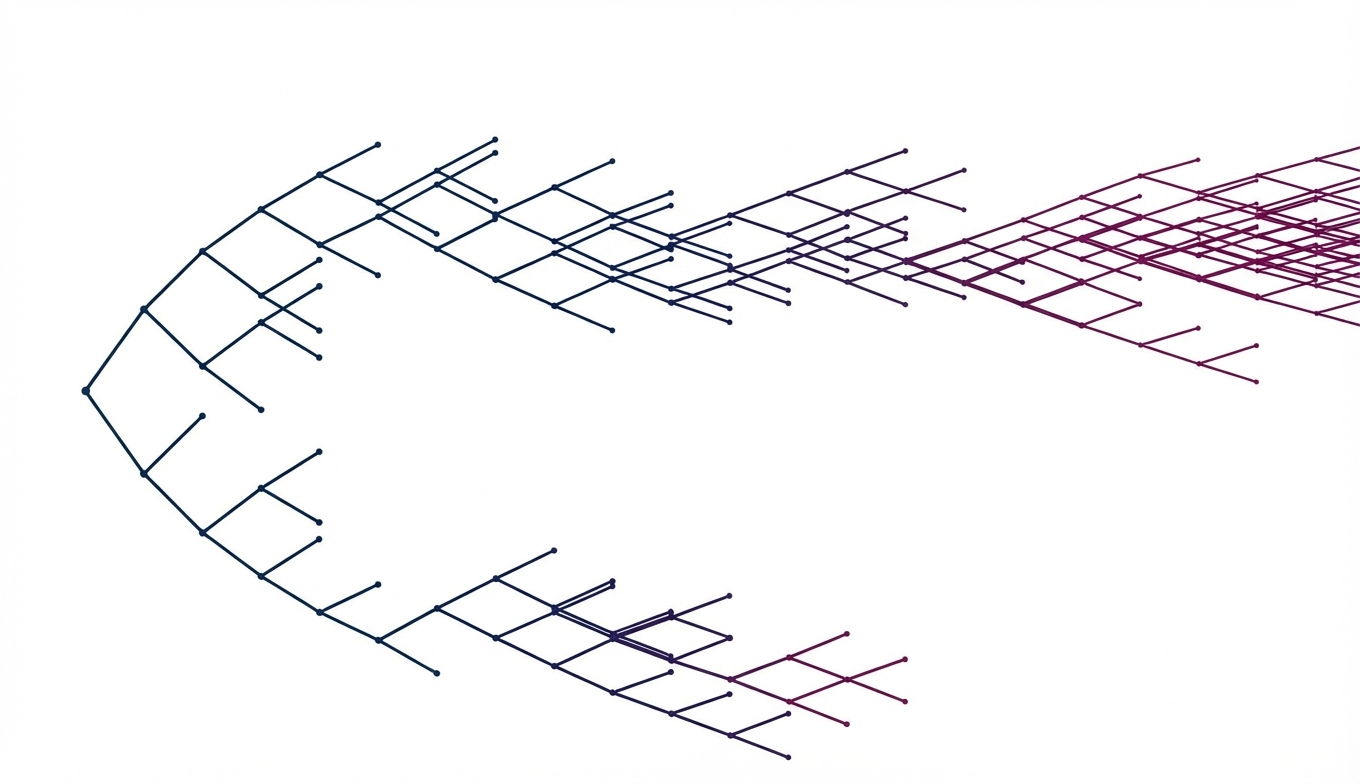
\includegraphics[width=0.78\textwidth]{figures/IMG_ch3/simpleGWvis.png}\\[6pt]
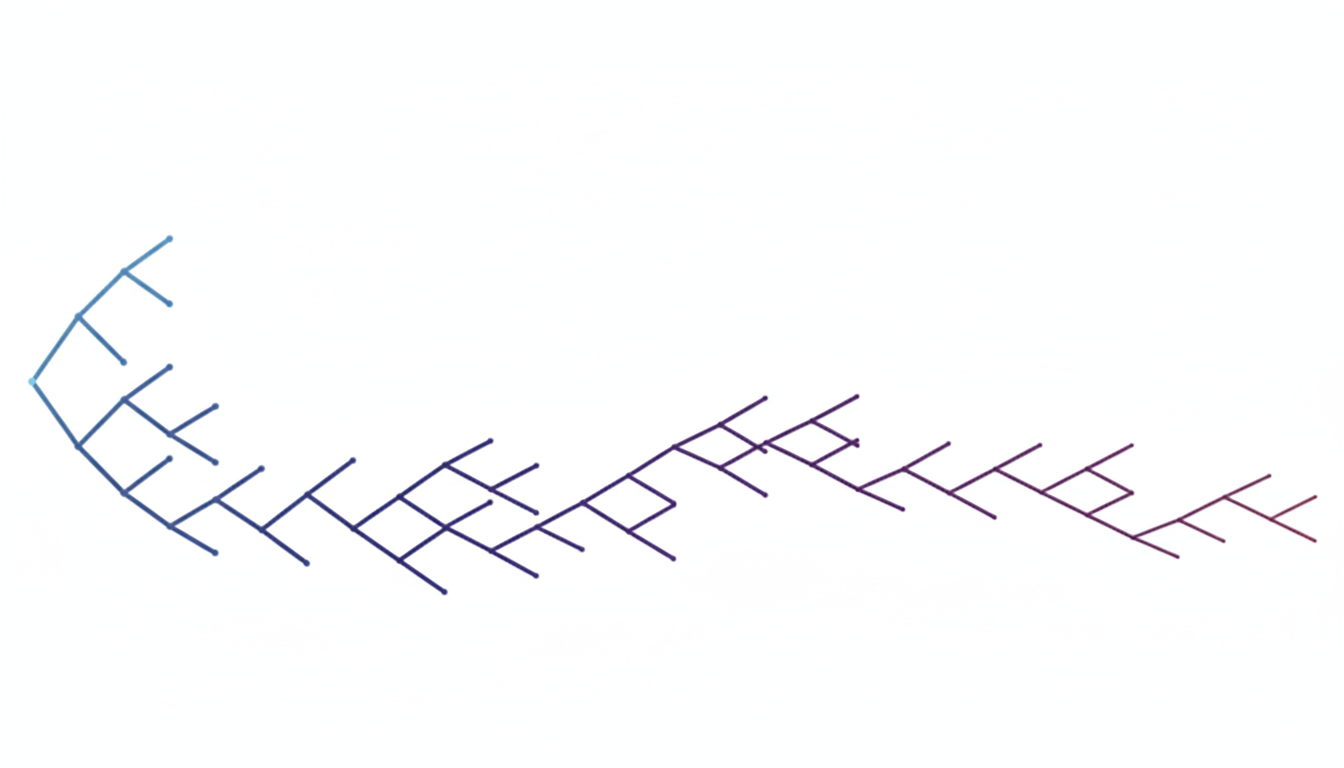
\includegraphics[width=0.78\textwidth]{figures/IMG_ch3/subGWvis.png}
\caption{Realisations of the simple Galton--Watson process, drawn as genealogies
with generation increasing to the right. Top: supercritical, $p=0.58$, where the
number of lines grows without bound. Bottom: subcritical, $p=0.47$; the same
construction, but the tree terminates. Colour encodes generation number.}
\label{fig:gwvis}
\end{figure}

\noindent
The offspring \pgf{} is
\begin{equation}
\label{eq:pgfbinary}
\phi(z) = \ex{z^{L}} = pz^2 + (1-p),
\end{equation}
so that \cref{eq:iterPGF} reads
\begin{equation}
\label{eq:unIter}
u_{n+1} = p\,u_n^2 + 1-p .
\end{equation}
The recursion has a direct combinatorial reading, and it is worth taking a moment
over it because the same argument recurs in \cref{sec:cohort,sec:bdc}. If the
founder dies at its first step, which happens with probability $1-p$, extinction
has already occurred. If instead it divides, with probability $p$, then extinction
by generation $n+1$ requires each of the two fresh lineages to die out within its
own $n$ generations, and those lineages are independent, so that happens with
probability $u_n^2$.

It is more convenient to work with the complement. Put
\begin{equation*}
S_n = 1-u_n = \pr{Z_n>0},
\end{equation*}
the probability that the process is still alive at generation $n$. Substituting
$u_n = 1-S_n$ into \cref{eq:unIter} and simplifying gives
\begin{equation}
\label{eq:SnIter}
S_{n+1} = 2pS_n - pS_n^2,\qquad S_0 = 1 .
\end{equation}
A population cannot return from extinction, so $u_n$ is non-decreasing and bounded
above by $1$; equivalently $S_n$ is non-increasing and bounded below by $0$, and
therefore converges to some $S_\infty\in[0,1]$.

\subsection{Certainty of extinction}
\label{sec:certainty}

Since $S_n$ converges, its limit must be a fixed point of \cref{eq:SnIter}. Setting
$S_{n+1}=S_n=S_\infty$,
\begin{equation*}
S_\infty = 2pS_\infty - pS_\infty^2
\qquad\Longleftrightarrow\qquad
p\,S_\infty\lrb{S_\infty + \tfrac1p - 2} = 0 ,
\end{equation*}
with roots
\begin{equation*}
S_\infty = 0
\qquad\text{and}\qquad
S_\infty = 2-\frac1p = \frac{2p-1}{p} .
\end{equation*}
For $p<\tfrac12$ the second root is negative and carries no probabilistic meaning,
so the only admissible limit is $S_\infty=0$ and extinction is certain. At
$p=\tfrac12$ the two roots collide at the origin and extinction remains certain.
For $p>\tfrac12$ a positive root appears, and it is that root which is attained:
the process survives forever with positive probability
$S_\infty = (2p-1)/p$. \Cref{fig:phase_transition} shows the transition, together
with the change in stability of the origin that produces it.

\begin{figure}[htbp]
    \centering
    \begin{subfigure}[b]{0.31\textwidth}
        \centering
        \begin{tikzpicture}
            \begin{axis}[ch2plotstyle]
                \addplot[blue, thick] {2*0.3*x - 0.3*x^2};
                \addplot[black!45, dashed] {x};
                \addplot[only marks, mark=*, red, mark size=1.6pt] coordinates {(0,0)};
            \end{axis}
        \end{tikzpicture}
        \caption{Subcritical ($p = 0.3$)}
    \end{subfigure}
    \hfill
    \begin{subfigure}[b]{0.31\textwidth}
        \centering
        \begin{tikzpicture}
            \begin{axis}[ch2plotstyle]
                \addplot[blue, thick] {2*0.5*x - 0.5*x^2};
                \addplot[black!45, dashed] {x};
                \addplot[only marks, mark=*, red, mark size=1.6pt] coordinates {(0,0)};
            \end{axis}
        \end{tikzpicture}
        \caption{Critical ($p = 0.5$)}
    \end{subfigure}
    \hfill
    \begin{subfigure}[b]{0.31\textwidth}
        \centering
        \begin{tikzpicture}
            \begin{axis}[ch2plotstyle]
                \addplot[blue, thick] {2*0.74*x - 0.74*x^2};
                \addplot[black!45, dashed] {x};
                \addplot[only marks, mark=*, red, mark size=1.6pt] coordinates {(0,0) (0.64865,0.64865)};
            \end{axis}
        \end{tikzpicture}
        \caption{Supercritical ($p = 0.74$)}
    \end{subfigure}

    \vspace{10pt}
    \begin{subfigure}[b]{0.55\textwidth}
    \centering
    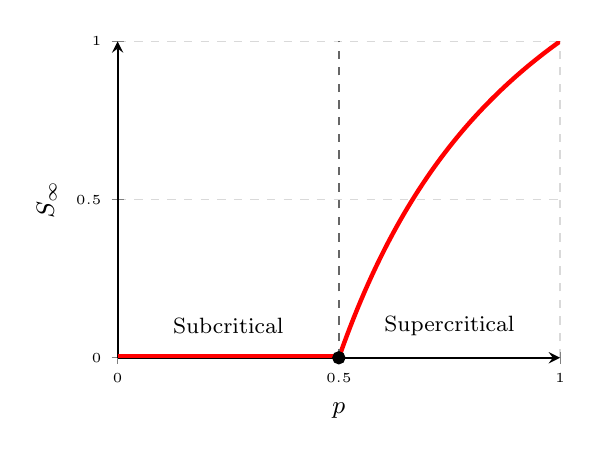
\begin{tikzpicture}
        \begin{axis}[
            width=7.2cm, height=5.6cm,
            axis lines=left,
            xlabel={$p$}, ylabel={$S_\infty$},
            xmin=0, xmax=1, ymin=0, ymax=1,
            xtick={0,0.5,1}, ytick={0,0.5,1},
            grid=major, grid style={dashed, gray!30}, thick,
            label style={font=\small}, tick label style={font=\tiny}
        ]
            \addplot[red, ultra thick, domain=0:0.5] {0.004};
            \addplot[red, ultra thick, domain=0.5:1, samples=120] {(2*x-1)/x};
            \draw[dashed, black!60] (axis cs:0.5,0) -- (axis cs:0.5,1);
            \node[font=\footnotesize] at (axis cs:0.25, 0.10) {Subcritical};
            \node[font=\footnotesize] at (axis cs:0.75, 0.10) {Supercritical};
            \addplot[only marks, mark=*, mark size=2pt, black] coordinates {(0.5,0)};
        \end{axis}
    \end{tikzpicture}
    \caption{The transition in $S_\infty$}
    \end{subfigure}

    \caption{Fixed points of the survival recursion \cref{eq:SnIter}. Panels
    (a)--(c) show the map $S\mapsto 2pS-pS^2$ (blue) against the diagonal (dashed),
    with the fixed points marked in red. Below and at criticality the origin is the
    only fixed point in $[0,1]$ and it is attracting, so extinction is certain; at
    $p=\tfrac12$ the map is tangent to the diagonal there. For $p>\tfrac12$ the
    origin turns repelling and a stable positive fixed point $S_\infty=(2p-1)/p$
    separates from it, traced in panel~(d). The survival probability is identically
    zero below the critical point and rises continuously above it.}
    \label{fig:phase_transition}
\end{figure}

\subsection{The critical case: a power law and an infinite expected lifetime}
\label{sec:criticalcase}

At $p=\tfrac12$ the expectation is constant, $\ex{Z_n}=1$ for every $n$, and yet
extinction is certain. The two facts are reconciled by the tail: rare realisations
survive for enormously long times and grow enormously large, and they do so at
exactly the rate needed to hold the mean at one. Demonstrating this is worth the
space, because the same calculation supplies the asymptotics of $S_n$ that
\cref{sec:Ap} will need.

Let
\begin{equation*}
T = \inf\{n : Z_n = 0\}
\end{equation*}
be the extinction time, so that the process passes through generations
$0,1,\dots,T-1$ and is dead at $T$. Writing $T$ as a sum of indicators and taking
expectations term by term --- legitimate because every term is non-negative ---
\begin{equation}
\label{eq:ETsumSn}
\ex{T} = \sum_{n=0}^{\infty}\pr{T>n} = \sum_{n=0}^{\infty}\pr{Z_n>0}
= \sum_{n=0}^{\infty}S_n .
\end{equation}
The question is therefore how fast $S_n$ decays at criticality.

Setting $p=\tfrac12$ in \cref{eq:SnIter} gives $S_{n+1}-S_n = -\tfrac12 S_n^2$.
Once $n$ is large the unit generational increment is small compared with the scale
on which $S_n$ varies, and the difference on the left is well approximated by a
derivative. This step is heuristic --- it replaces a difference equation by a
differential one, and nothing here justifies the replacement beyond the smallness
of the increment relative to the solution --- but its conclusion is standard and is
confirmed by simulation below. With that caveat,
\begin{equation*}
\dda{S}{n} = -\tfrac12 S^2,
\qquad\text{with general solution}\qquad
S(n) = \frac{2}{n+\text{const}},
\end{equation*}
so that
\begin{equation}
\label{eq:twoovern}
S_n \sim \frac{2}{n}\qquad(n\to\infty),
\end{equation}
as \cref{fig:power_law}(a) confirms. Substituting into \cref{eq:ETsumSn}, the tail
of the sum behaves like twice the harmonic series,
\begin{equation*}
\ex{T} = \sum_{n=0}^{\infty}S_n \sim \sum_{n=1}^{\infty}\frac{2}{n},
\end{equation*}
which diverges (\cref{fig:harmonic}). Since every $S_n$ is positive,
$\ex{T}=\infty$: the expected lifetime of the critical Galton--Watson process is
infinite even though extinction occurs with probability one.

\begin{figure}[H]
    \centering
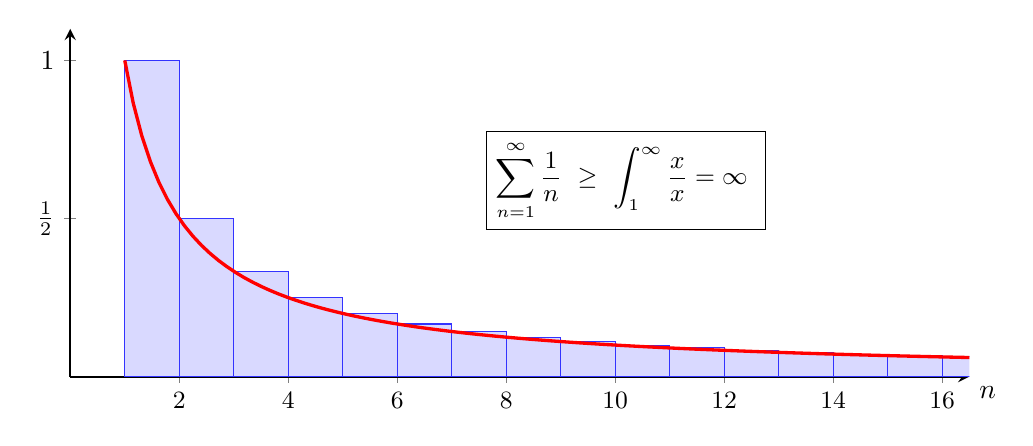
\begin{tikzpicture}
    \begin{axis}[
        axis lines = middle,
        xmin = 0, xmax = 16.5, ymin = 0, ymax = 1.1,
        xlabel = {$n$},
        xtick = {2,4,6,8,10,12,14,16},
        ytick = {0.5, 1}, yticklabels = {$\frac{1}{2}$, $1$},
        axis line style = {thick},
        width = 13cm, height = 6cm,
        every axis x label/.style={at={(current axis.right of origin)}, anchor=north west},
        xticklabel style={font=\small},
    ]
        \addplot[fill=blue!15, draw=blue!80, ybar interval, samples at={1,2,...,17}] {1/x} \closedcycle;
        \addplot[red, domain=1:16.5, samples=100, very thick] {1/x};
        \node[draw, fill=white, align=left, font=\small] at (axis cs: 10.2, 0.62) {
            $\displaystyle \sum_{n=1}^{\infty} \frac{1}{n} \ \ge\ \int_{1}^{\infty} \frac{\dd x}{x} = \infty$
        };
    \end{axis}
\end{tikzpicture}
\caption{Divergence of the harmonic series. Each blue rectangle has area $1/n$ and
contains the region under the red curve $1/x$ on $[n,n+1]$, so the sum of the areas
exceeds $\int_1^\infty x^{-1}\dd x=\infty$. Because $S_n\sim2/n$ at criticality,
the same divergence carries over to $\ex{T}=\sum_nS_n$.}
\label{fig:harmonic}
\end{figure}

The heavy tail responsible is visible directly in simulation. A power-law
distributed quantity carries a modest but non-negligible chance of an
extraordinarily large realisation, and a sample mean computed from such a quantity
does not settle: the larger the sample, the larger the mean, because the occasional
enormous value keeps pushing the normalised sum upward. \Cref{fig:power_law}
collects the three classical critical exponents --- for the survival probability,
for the extinction time and for the total progeny.

\begin{figure}[ht]
    \centering
    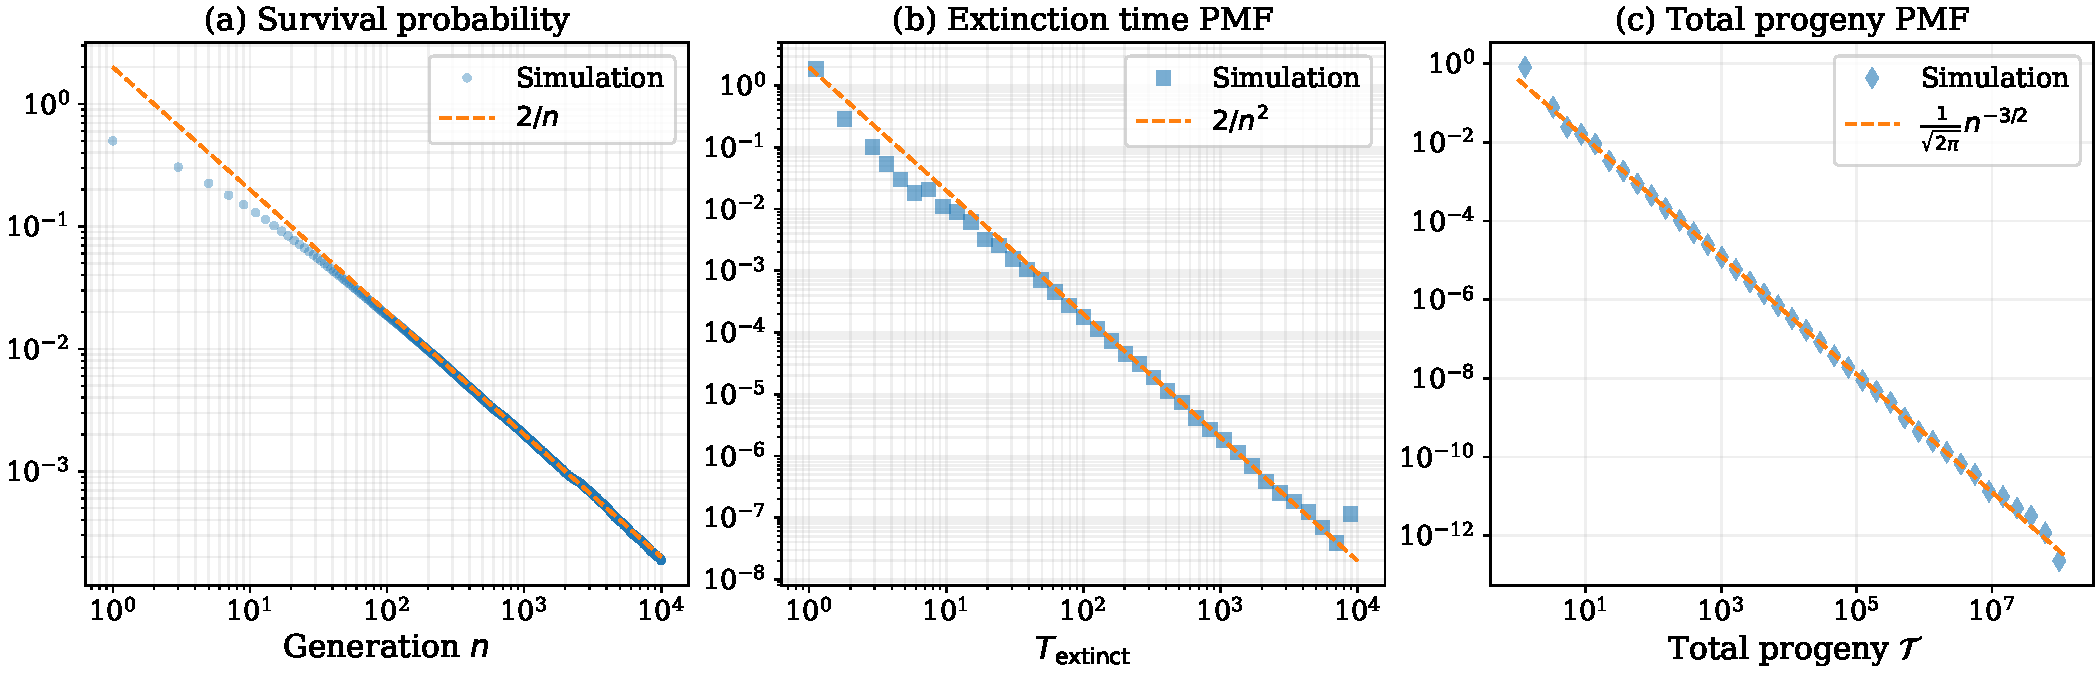
\includegraphics[width=0.98\textwidth]{figures/IMG_ch3/power_law_fixed.pdf}
    \caption{Power-law behaviour in the critical Galton--Watson process
    ($p=0.5$), from $10^6$ realisations.
    (a) Survival probability $S_n=\pr{Z_n>0}$, showing the late-generation scaling
    $S_n\sim2/n$ of \cref{eq:twoovern}.
    (b) Probability mass function of the extinction time $T=\inf\{n:Z_n=0\}$, with
    heavy tail $\pr{T=n}\sim2/n^2$.
    (c) Probability mass function of the total progeny
    $\mathcal T = \sum_{k\ge0}Z_k$, displaying the classical critical branching
    asymptotic $\pr{\mathcal T=n}\sim n^{-3/2}$.}
    \label{fig:power_law}
\end{figure}

\FloatBarrier
